\documentclass{homework}
\author{Maya Basu}
\class{Analytic Mechanics}
\title{Class Notes}

\newcommand{\inte}{\text{Int}}
\newcommand{\clos}[1]{\overline{#1}}
\newcommand{\RR}{\mathbb{R}}
\newcommand{\BB}{\mathbb{B}}
\newcommand{\MM}{\mathbb{M}}
\newcommand{\OO}{\mathbb{O}}
\newcommand{\m}[1]{\begin{bmatrix} #1 \end{bmatrix}}
\newcommand{\kt}{\rangle}
\newcommand{\br}{\langle}
\newcommand{\ket}[1]{| #1 \rangle}
\newcommand{\bra}[1]{ \langle #1 |}
\begin{document} \maketitle
\section{Constants}


\section{Postulates of Quantum Mechanics}
\begin{enumerate}
    \item The state of a quantum mechanical system, including all the information you can know about it, is represented mathematically by a normalized $| \psi \kt$ 
    \item A physical observable is represented mathematically by an operator $A$ that acts on kets.
    \item The only possible result of a measurement of an observable is one of the eigenvalues $a_n$ of the corresponding operator $A$.
    \item The probability of obtaining the eigenvalue a system in the state $| \psi \kt$  is in a measurement of the observable A on the $\mathbb{P}_{a_n} = |\br a_n | \psi_{in} \kt |^2$ where $a_n$ is the normalized eignvector of $A$ corresponding to an eignvalue $a_n$
    \item After a measurement of $A$ that yields the result $a_n$, the quantum system is in a new state that is the normalized projection of the original system ket onto the ket (or kets) corresponding to the result of the measurement, $| \psi' \kt = \frac{P_n | \psi \kt}{\sqrt{ \br \psi | P_n | \psi \kt}}$
    \item The time evolution of a quantum system is determined by the Hamiltonian or total energy operator $H(t)$ through the Schrödinger equation $i\hbar \frac{d}{dt}| \psi (t) \kt = H(t)| \psi (t) \kt$


\end{enumerate}


\section{Classical torque on a magnetic (dipole) moment in a magnetic field}

\subsection{$\vec{B}$ is uniform}

Suppose we have a tilted loop of current in a magnetic field, with it's area vector at an angle $\theta$ from the magnetic field. The force on one unit of charge going around this loop is $\vec{F} = q\vec{v} \times \vec{B}$. If we track a positive charge around this loop we note that there is a troque which rights the loop. However, in a uniform magnetic field, there is no net force. 

\subsection{$\vec{B}$ is non uniform}

Suppose that the magnetic field points along the $z$ direction with a nonzero gradient $\frac{dB_z}{dz}>0$. This alone does not cause a force on the loop. However, Maxwelll's equations dictate that the divergence of the magnetic field must be $0$, so if $\frac{dB_z}{dz}>0$ then the magnetic field must have non zero partial derivatives in $x$ and $y$ which exert an overall force in the positive $z$ direction (for positive charge). The potential energy is $E = -\vec{m}\cdot \vec{B}$ so the force is $ \vec{\nabla} (\vec{m} \cdot \vec{B})$ which is $m_z\frac{dB_z}{dz}$ along the $z$ axis.


\subsection{Magnetic moment and classical angular momentum}

We can model the magnetic moment of an atom as coming from a circling electron. The current is charge/time, $\frac{-e}{\text{orbit time}} = \frac{-ev}{2\pi r}$. The magnetic moment of this loop is $I$ times the area vector, or $\frac{-e}{2}vr = \frac{-e m_e vr}{2m_e} = \frac{-e}{2m_e}L$ so $\vec{m} = \frac{-e}{2m_e}\vec{L}$. 


\section{Stern-Gerlatch Experiment}

In the case of the classical dipole, we had a force along the $z$ direction equal to $m_z\frac{dB_z}{dz}$. So in the $z$ varying magnetic field of the stern gerlatch experiment, the force is proportional to the $z$ component of the magnetic dipole moment of the atoms, which we expect to take on an even distribution. However, when atoms are put through the device they end up being measured with discrete values of the $z$ component of their angular momentum. Differetn atoms lead to different outcomes. 

\subsection{Silver}

In the case of silver, the lone outermost elecron does not have orbital angular momentum, but it does have spin, which is some intrinsic angular momentum. Taking the calculation with orbital angular momentum as an analogy, we have $\vec{m} = \frac{-g_s \mu_B \vec{S}}{\hbar}$ where $\mu_B = \frac{e \hbar}{2m_e}$, $\vec{S}$ is the angular momentum and $g_s$ is very close to $2$ and comes from an integral over the charge distribution (since we are dealing with intrinsic spin instead of orbital angular momentum) (in fact this was historically measured as $m_z = \pm \mu_B$). Along the $z$ axis, $S_z = \pm \frac{\hbar}{2}$.

\subsection{Other atoms than silver}

Generally, the projection of angular momentum onto an axis $\vec{J} \cdot \vec{n}$ comes in values separated by $\hbar = \frac{h}{2\pi}$

\section{Braket notation}

Postulate of quantum mechanics: 
All information about the state can be summarized in a normalized ket $\br \psi | \psi \kt = 1$. 
The probability of detecting a state (abreviated as $P_x$) such as $| + \kt$ is $| \br + | \psi \kt |^2$ (this is the conventional order)

If $|\psi \kt = a | + \kt + b | - \kt$ then $\br \psi | = a^* \br \psi | + b^* \br \psi |$
In general, $\br \psi | \phi \kt = \br  \phi | \psi \kt^*$

Basis vectors such as $| \pm_z \kt$ must be orthonormal and complete (meaning they span the hilbert space)

For a general quantum system, we have 
$\br a_i | a_j \kt = \delta_{ij}$ (orthogonality)
$| \psi \kt = \sum_i \bra a_i | \psi \kt |a_i \kt$
Or
$\sum_n P_{a_n} = \sum_n |a_n \kt \br a_n | = 1$ (sum of projections is the identity)
And the probability of measuring this system in a state is 
$P_{a_n} = |\br a_n | \psi_{in} \kt|^2$


\[| +_x \kt = \frac{1}{\sqrt{2}}[|+_z \kt + |-_z \kt] = \frac{1}{\sqrt{2}} \m{ 1\\ 1}\]
\[| -_x \kt = \frac{1}{\sqrt{2}}[|+_z \kt - |-_z \kt]= \frac{1}{\sqrt{2}} \m{ 1\\ -1}\]

\[| +_z \kt = \frac{1}{\sqrt{2}}[|+_x \kt + |-_x \kt] =  \m{ 1\\ 0}\]
\[| -_z \kt = \frac{1}{\sqrt{2}}[|+_x \kt - |-_x \kt] = \m{ 0\\ 1}\]

\[| +_y \kt = \frac{1}{\sqrt{2}}[|+_z \kt + i|-_z \kt] = \frac{1}{\sqrt{2}} \m{ 1\\ i}\]
\[| -_y \kt = \frac{1}{\sqrt{2}}[|+_z  \kt - i|-_z \kt] = \frac{1}{\sqrt{2}} \m{ 1\\ -i}\]
\[| \psi  \kt = \m{\br +_z|\psi \kt \\ \br -_z|\psi \kt}\]

These are all super position states, sometimes called "coherent" superpositions, because the relative phase is important (such as the sign in $| \pm_x \kt$ determining the measurement along the $x$ basis).


\begin{figure}[htp]
    \centering
    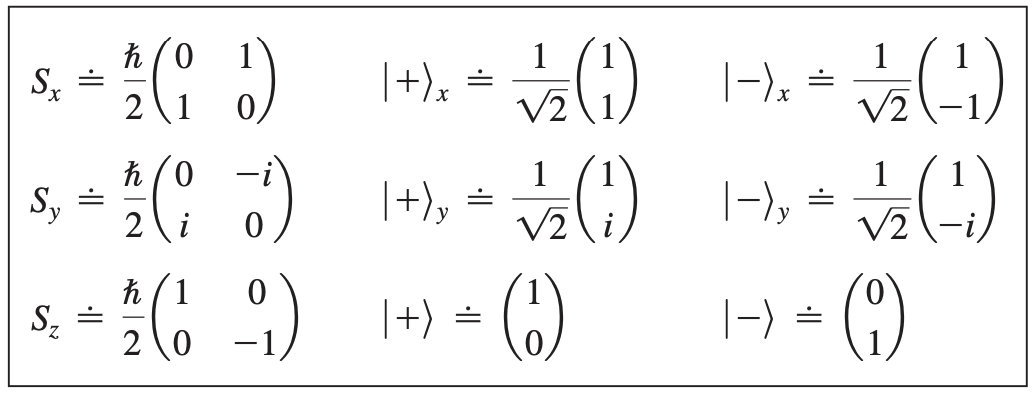
\includegraphics[width=12cm]{mreps.png}
   

\end{figure}
\section{Operators}

Observables are represented by operators, which act on kets to produce other kets. For the eign vectors of an observable, the kets are only multiplied by a constant. The eignvalues corresponding to these eign vectors are the only possible values of a measurement of that observable.
In their own basis, operators are diagonal since eign values are unit vectors in their own basis.
\[S_z = \m{\hbar/2 & 0 \\ 0 & -\hbar/2}\]
\[S_x = \m{  0 & \hbar/2 \\ \hbar/2 & 0}\]
\[S_y = \m{ 0 & -i\hbar/2\\ i\hbar/2 & 0 }\]



We can isolate a matrix element of an oporator by sandwitching it between two of it's basis vectors:
\[A = \m{\br + | A | + \kt & \br + | A | - \kt \\ \br - | A | + \kt & \br - | A | - \kt}\]
Or generally, $A_{ij} = \br i | A | j \kt$
This is still called a matrix element even when the ket and bra are not basis vectors.

\section{The general direction}
\[ \hat{n} = \hat{i}\sin(\theta)\cos(\phi)+ \hat{j}\sin(\theta)\sin(\phi) + \hat{k}\cos(\theta)\]

\begin{figure}[htp]
    \centering
    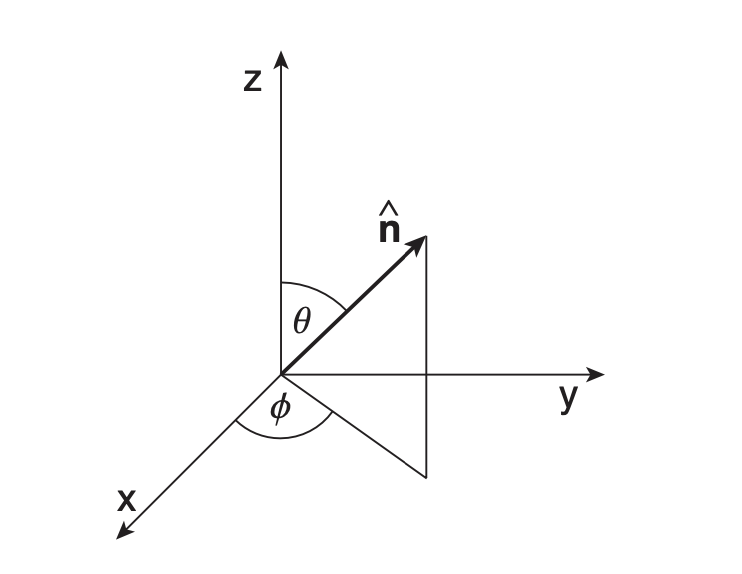
\includegraphics[width=4cm]{sphericalangles}
    \caption{$0 \leq \theta < \pi$, $0 \leq \phi < 2\pi$}

\end{figure}


And $S_n = S \cdot \hat{n} = S_x\sin(\theta)\cos(\phi)+ S_y\sin(\theta)\sin(\phi) + S_z\cos(\theta)$

We can also represent this as a matrix:
\[S_n  = \frac{\hbar}{2}\m{\cos(\theta) & \sin(\theta)e^{-i\phi} \\\sin(\theta)e^{i\phi} & -\cos(\theta)}\]
with eign vectors
\[\ket{+_n} = \cos \frac{\theta}{2}\ket{+} + \sin \frac{\theta}{2}e^{i\phi}\ket{-}\]
\[\ket{-_n} = \sin \frac{\theta}{2}\ket{+} - \cos \frac{\theta}{2}e^{i\phi}\ket{-}\]


\subsection{Finding Eignvalues and Eignvectors}

To find the eign values we can use the equation $\det(A - \lambda I) = 0$

The equation for the eign vectors of an operator $A$ is 

\[\m{A_{11} & A_{12} \\ A_{21} & A_{22}}\m{c_{n1} \\ c_{n2}} = a_n \m{c_{n1} \\ c_{n2}}\]
which multiplies out to the equations
\[(A_{11} - a_n)c_{n1} + A_{12}c_{n2} = 0\]
\[A_{21}c_{n1}+ (A_{22}- a_n)c_{n2} = 0\]


\section{Hermition-ness}

If $A \ket{a} = \ket{b}$, then the corresponding bra is $\bra{b} = \bra{a}A^{\dag}$. Where $\dag$ is the conjugated transpose, and we say $H$ is hermitian if $H^{\dag} = H$.


\section{Projection Operators}

We can write any state as 
\[\ket{\psi} = \bra{+}\psi \rangle \ket{+} + \bra{-}\psi \rangle \ket{-} \]
Because of the completness of this basis. But these inner products are just numbers, so we can shift to get
\[\ket{\psi} = \ket{+}\bra{+}\psi \rangle  +  \ket{-} \bra{-}\psi \rangle = (\ket{+}\bra{+}  +  \ket{-} \bra{-}) \ket{\psi}\]
Representing as matrices, we see
\[P_{+} =\ket{+}\bra{+}  = \m{1 & 0 \\ 0 & 0 }\]
\[P_{-} =\ket{-}\bra{-}  = \m{0 & 0 \\ 0 & 1 }\]


\section{Expected value}

The expected value of an oporator is 
\[\langle A \rangle = \langle \psi | A | \psi \rangle = \sum_{n}a_nP_{a_n}\]
Where $a_n$ are the eign vectors and $P_{a_n} = |\bra{a_n} \psi \rangle|^2$ is the probability of measureing $a_n$. 

We can define the rms (root mean squared) deviation of $A$ as follows
\[\Delta A = \sqrt{\langle (A - \langle A \rangle)^2 \rangle} = \sqrt{\langle A^2 \rangle  - \langle A \rangle^2}\]

where $\langle A^2 \rangle$ can be calculated as $\langle \psi | A^2 | \psi \rangle$ where $A^2 \psi = A(A(\psi))$

\section{Commutation}

Define the commuter of two oporators to be $[A,B] = AB - BA$, we say $A$ and $B$ commute iff this is $0$.

If $A$ and $B$ commute, then for an eign vector of $A$, we have $A | a \kt = a | a \kt$, $BA | a \kt = aB | a \kt$, $A(B| a \kt) = a(B| a \kt)$, so $B| a \kt$ is an eign vector of $A$, and it must be the same eign vector as $| a \kt$, since they share eignvalues (disregarding degeneracy), so $B| a \kt = b| a \kt$, or $| a \kt$ is also an eign vector of $B$. - So commuting operators share common eignvalues

WHen $A$ and $B$ commute we call them compatable - if we measure $A$ we end up with a projection onto a $| a \kt$. But since this is also an eign state of $B$, measuring $B$ also gives $| a \kt$ so we can measure $A$ again and get back $| a \kt$, measuring $B$ does not destroy information about $A$, so we can know the eign values of both observables simultaneously.

If two matrices are both diagonal in the same basis then they both commute - matrices are diagonal in their own basis - and we can see the order doesn't matter between two diagnonal matrices. However, if one or more is not diagonal that does not mean they do not commute


\subsection{Angular Momentum Commutation relations}
\[[S_x,S_y] = i \hbar S_z\]
\[[S_y,S_z] = i \hbar S_x\]
\[[S_z,S_x] = i \hbar S_y\]



\section{Uncertainty Principle}

The uncertainty principle states that the product of uncertainties or standard deviations of two observables is 
\[\Delta A \Delta B \ge \frac{1}{2}|\br [A,B] \kt|\]


\section{The $S^2$ operator}

We can consider the operator 
\[S^2 = S_x^2 + S_y^2 + S_z^2 = \frac{3}{4}\hbar^2\m{1 & 0 \\ 0 & 1}\]

This is proportional to the identity operator, so $S^2 \ket{\psi} = \frac{3}{4}\hbar^2\ket{\psi}$ for all $\psi$. Since $\langle S^2 \rangle = \frac{3}{4}\hbar^2$ for the spin 1/2 system, then the "length" of the spin state is $\sqrt{3}\frac{\hbar}{2}$

\section{Spin $1$ systems}

The eign vectors are $\ket{-1}, \ket{0} \ket{1}$ with eign values $-\hbar, 0, \hbar$ respectiely. SO in matrix representation this becomes
\[S_z = \hbar \m{1 & 0 & 0 \\ 0 & 0 & 0 \\ 0 & 0 & -1}\]

\begin{figure}[htp]
    \centering
    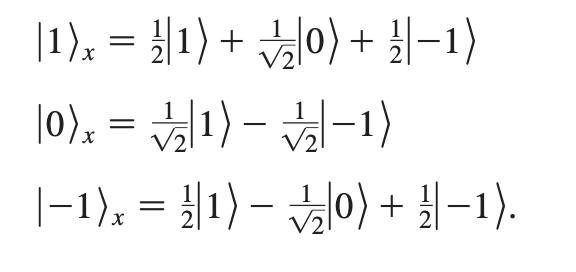
\includegraphics[width=12cm]{Sx}
   

\end{figure}
\begin{figure}[htp]
    \centering
    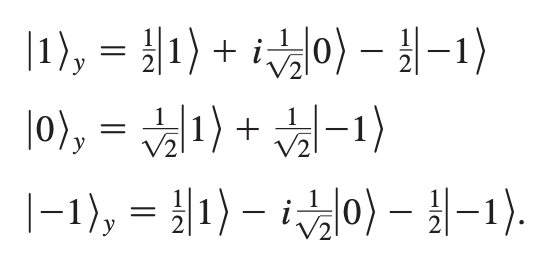
\includegraphics[width=12cm]{Sy}
   

\end{figure}
\begin{figure}[htp]
    \centering
    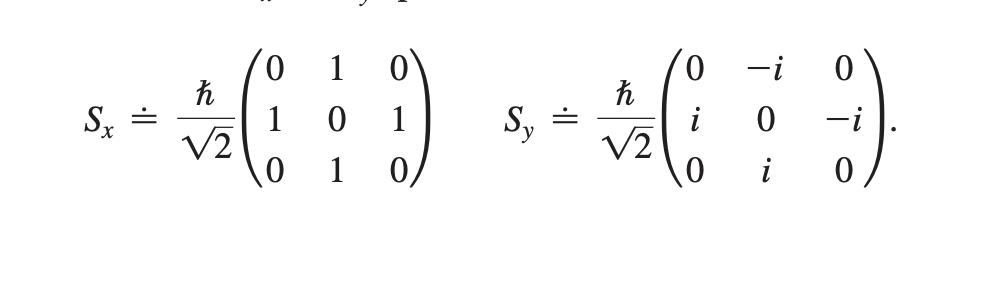
\includegraphics[width=12cm]{Sxymatrices}


\end{figure}




\section{Time Evolution}

Via a postulate, time evolution is governed by 
\[i\hbar \frac{d}{dt}\ket{\psi(t)} = H(t)\ket{\psi(t)}\]
Generally, we want to express $\ket{\psi}$ in terms of the energy eign basis, or the basis of eignvectors of $H$ as in $\ket{\psi} = \sum_n c_n(t)\ket{E_n}$, then (we see this by substituting in and using the fact these are eign vectors) we get
\[\ket{\psi(t)} = \sum_n c_n(t)e^{-iE_nt/\hbar}\ket{E_n}\]
and we call $\omega_{ab} = \frac{E_a - E_b}{\hbar}$



\section{Spin Procession}
 
Recall that the magnetic moment is $\mu = g \frac{q}{2m_e}S$ and the (classical) hamiltonian is $H = - \mu \cdot B = \frac{e}{m_e}S \cdot B$ if we substitute $q = -e$ and $g= 2$ (not actually $2$).


\subsection{Magnetic field pointing in the $z$ direction}
We can then consider a specific magnetic field. For example, for a magnetic field in the $z$ direction $B = B_0\hat{z}$ we get
\[H = \frac{eB_0}{m_e}S_z = \omega_0S_z = \frac{\hbar \omega_0}{2}\m{1&0\\0& -1}\]
when $\omega_0 = \frac{eB_0}{m_e}$ is the "angular frequency". A general state 
\[\ket{\psi} = \ket{+_n} = \cos \frac{\theta}{2}\ket{+} + \sin \frac{\theta}{2}e^{i\phi}\ket{-} \]
or
\[\ket{\psi(0)} = \m{\cos \theta/2 \\ e^{i \phi}\sin \theta/2}\]
Then for a magnetic field in the $z$ direction, this is already in the energy eignbasis so 
\[\ket{\psi(t)} = \m{e^{-i\omega_0t/2}\cos \theta/2 \\ e^{i\omega_0t/2}e^{i \phi}\sin \theta/2} = e^{-i\omega_0t/2}\m{\cos \theta/2 \\ e^{i (\phi + \omega_0t)}\sin \theta/2}\]
and if we calculate the probability of measuring spin up, we get $\cos{\theta/2}$. This is time independent since $H$ and $S_z$ commute. However, for $x$ we get $\frac{1}{2}[1 + \sin \theta \cos(\phi + \omega_0t)]$

Calculating the expectation values for these, we get $\langle S_z \rangle = \frac{\hbar}{2}\cos \theta$ and $\langle S_x \rangle = \frac{\hbar}{2}\sin \theta \cos (\phi + \omega_0t)$ (This is called Larmor precession and the frequency is the Larmor frequency)

\section{Magnetic Field in a general direction}

Suppose we have $B = B_0\hat{z} + B_1\hat{x}$. Then we define Larmor frequencies for both directions - $\omega_0 = \frac{eB_0}{m_e}$, and $\omega_1 = \frac{eB_1}{m_e}$ so the hamiltonian becomes 
\[H = \omega_0S_z + \omega_1S_x = \frac{\hbar}{2}\m{\omega_0 & \omega_1 \\ \omega_1 & -\omega_0}\]
Diagonalizing this gives eign values $\pm\frac{\hbar}{2}\sqrt{\omega_0^2 + \omega_1^2}$
This is pointing in the direction

\begin{figure}[htp]
    \centering
    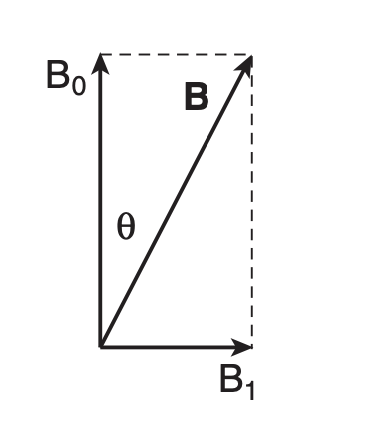
\includegraphics[width=4cm]{direction.png}
\end{figure}

So we can write
\[H = \frac{\hbar}{2}\sqrt{\omega_0^2 + \omega_1^2}\m{\cos \theta & \sin \theta \\ \sin \theta & -\cos \theta}\]
Now we can consider how a specific state evolves in this field

\section{Spin flip}

Suppose the state starts as $\ket{\psi(0)} = \ket{+_z}$ we can write this as $\ket{\psi(0)} = \cos \frac{\theta}{2} \ket{+_n} + \sin \frac{\theta}{2} \ket{-_n}$ using the eign states for the arbitrary direction. Since this is the energy eign basis we can write it as
\[\ket{\psi(t)} = e^{iE_+t/\hbar}\cos \frac{\theta}{2} \ket{+_n} + e^{iE_-t/\hbar}\sin \frac{\theta}{2} \ket{-_n}\]
with $E = \pm \frac{\hbar}{2}\sqrt{\omega_0^2 + \omega_1^2}$ We can take the magnitude squared of the inner product of this with the $-$ state to get the probability of a spin flip as 
\[P_{+ \rightarrow -} = \frac{\omega_1^2}{\omega_1^2 + \omega_0^2}\sin^2 \left(\frac{\sqrt{\omega_0^2 +\omega_1^2}}{2}t \right)\]
(Rabi equation)


\section{Magnetic resonance}

Suppose that there is some magnetic field and a magnetic moment (classically) precessing around. If we go into a frame rotating with this moment, then it apears to be stationary which means there is no field and so even the slightest perpendicular fild with cause it to flip eventually. Suppose that the axes of precession is vertical, then in the rotating frame, we can apply a small magnetic field to flip this. Since this would be stationary in the rotating frame, in the stationary frame it looks like
\[B = B_1\cos(\omega t)\hat{x} + B_1\sin(\omega t)\hat{y}\]
Where if we allow $\omega \neq \omega_0$ then this would mean there is some residual rotation 
So now lets consider this field
\[B =B_0 \hat{z} + B_1[\cos(\omega t)\hat{x} + \sin(\omega t)\hat{y}]\]
The hamiltonian is
\[B =B_0 S_z + B_1[\cos(\omega t)S_x + \sin(\omega t)S_y\]
and we again define the Larmor frequencies $\omega_0 = \frac{eB_0}{m_e}$, $\omega_1 = \frac{eB_1}{m_e}$. Representing this as a matrix gives
\[H = \frac{\hbar}{2}\m{\omega_0 & \omega_1e^{-i\omega t}\\ \omega_1e^{i\omega t} & -\omega_0}\]
To solve this we want to convert to a rotating frame (not derived, just given as)
\[\ket{\tilde{\psi(t)}} \]
and a new hamiltonian as
\[\tilde{H} = \frac{\hbar}{2}\m{-\Delta \omega & \omega_1 \\\omega_1 & \Delta \omega} \]
where $\delta\omega = \omega  - \omega_0$. Notice this is time independant! So suppose the state starts in the state $\ket{+}$, then the probability of a spin flip is $\frac{\omega_1^2}{(\omega - \omega_0^2) + \omega_1^2}\sin^2(\frac{\sqrt{(\omega - \omega_0)^2 + \omega_1^2}}{2}t)$






\section{Shrodinger Equation with a Time Independant Hamiltonian}

In one dimensions we have
\[i\hbar \frac{d}{dt}\psi(x,t) = -\frac{\hbar^2}{2m}\frac{\delta^2}{\delta x^2}\psi(x,t) + V(x)\psi(x,t)\]
Lets try a solution of the form $\psi(x,t) = \psi(x)f(t)$:
\[i\hbar \psi(x)f'(t) = -\frac{\hbar^2}{2m}\psi''(x)f(t) + V(x)\psi(x)f(t)\]
\[i\hbar f'(t)/f(t) = [-\frac{\hbar^2}{2m}\psi''(x) + V(x)\psi(x)]/\psi(x)\]
\[i\hbar f'(t)/f(t) = [H\psi(x)]/\psi(x) = E\]
for some constant $E$ (both sides must be constant or else this relation can not hold. Then we have $f(t) = f(0)e^{-iEt/\hbar}$ and $\psi$ is an energy eign state of the hamiltonian. So for the time independant hamiltonian, we have
\[\psi(x,t)  = \sum_{n}c_n\psi_{E_n}e^{-iEt/\hbar}\]
since the eign states $\psi_{E_n}$ form a complete basis. 


\section{Infinite square well}







\end{document}




